\section{百发百中}
\markboth{3. 百发百中}{3. 百发百中}

人们常用“百发百中”来赞美神枪手。但是我们这里说的“百发百中”，却是指一个有趣的小游戏。

如图 3.1，用硬纸做一个椭圆形的盒子，并且在椭圆形盒底的一个焦点上放一粒钮扣，作为子弹，在另一个焦点处竖立一个钢笔套，作为靶子。你不需要瞄准，把钮扣子弹沿着盒底面内的任何方向弹射出去，经过盒壁反射后，都一定命中靶子，真是不折不扣的百发百中呢！

\begin{center}
  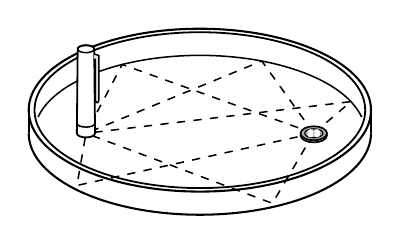
\begin{tikzpicture}[scale=1.05]
    % 椭圆形硬纸盒斜投影: 内底半轴 a=2.0, b=0.9425, 焦点 F1=(-1.3775, 0), F2=(1.3775, 0)
    \def\a{2.0}
    \def\b{0.9425}
    \def\c{1.3775}
    \def\h{0.28}

    % 盒外壁底部可见弧与两侧垂线
    \draw[line width=0.75pt] (-2.07,0) arc[start angle=180, end angle=360, x radius=2.07, y radius=0.985];
    \draw[line width=0.75pt] (-2.07,0) -- (-2.07,\h);
    \draw[line width=0.75pt] (2.07,0) -- (2.07,\h);
    % 盒顶外沿与内沿
    \draw[line width=0.75pt, fill=white] (0,\h) ellipse [x radius=2.07, y radius=0.985];
    \draw[line width=0.65pt, fill=white] (0,\h) ellipse [x radius=\a, y radius=\b];
    % 盒内壁底面可见弧(后半弧)
    \draw[line width=0.55pt] ({\a*cos(12)},{\b*sin(12)}) arc[start angle=12, end angle=168, x radius=\a, y radius=\b];

    \coordinate (F1) at (-\c, 0);
    \coordinate (F2) at (\c, 0);

    % 精确椭圆反射路径: 从 F2 射向盒底内壁 W(t), 反射至 F1
    \foreach \t in {24, 68, 118, 222, 296} {
      \coordinate (W) at ({\a*cos(\t)}, {\b*sin(\t)});
      \draw[dashed, line width=0.55pt] (F2) -- (W) -- (F1);
    }

    % 焦点 F2 处的四孔钮扣
    \begin{scope}[shift={(F2)}]
      \draw[fill=gray!25, line width=0.6pt] (0,-0.025) ellipse [x radius=0.16, y radius=0.085];
      \draw[fill=gray!65, line width=0.6pt] (0,0) ellipse [x radius=0.16, y radius=0.085];
      \draw[line width=0.4pt] (0,0) ellipse [x radius=0.11, y radius=0.055];
      \fill[white] (-0.04,0.015) circle (1.0pt) (0.04,0.015) circle (1.0pt)
                   (-0.04,-0.015) circle (1.0pt) (0.04,-0.015) circle (1.0pt);
    \end{scope}

    % 焦点 F1 处竖立的钢笔套(带笔夹)
    \begin{scope}[shift={(F1)}]
      \draw[fill=white, line width=0.65pt]
        (-0.11,0) arc[start angle=180, end angle=360, x radius=0.11, y radius=0.05]
        -- (0.10,1.02) arc[start angle=0, end angle=180, x radius=0.10, y radius=0.045]
        -- cycle;
      \draw[line width=0.55pt] (0,1.02) ellipse [x radius=0.10, y radius=0.045];
      \draw[line width=0.55pt] (-0.108,0.12) arc[start angle=180, end angle=360, x radius=0.108, y radius=0.045];
      \draw[fill=gray!20, line width=0.55pt]
        (0.10,0.96) -- (0.155,0.94) -- (0.155,0.40) arc[start angle=0, end angle=-180, x radius=0.02, y radius=0.03] -- (0.115,0.89) -- (0.10,0.90);
    \end{scope}
  \end{tikzpicture}
  \par\vspace{4pt}{\footnotesize 图\ 3.1}
\end{center}

\begin{wrapfigure}{r}{0.43\textwidth}
  \centering
  \vspace{-6pt}
  \begin{tikzpicture}[scale=1.05]
    \begin{scope}[rotate=-6]
      \def\a{1.55}
      \def\b{0.85}
      \def\c{1.2961}
      \coordinate (F1) at (-\c,0);
      \coordinate (F2) at (\c,0);
      \coordinate (P) at ({\a*cos(48)},{\b*sin(48)});
      \coordinate (T) at ($(P) + (-1.15, 0.568)$);
      \coordinate (TR) at ($(P) + (0.95, -0.469)$);
      \coordinate (N) at ($(P) + (-0.52, -1.053)$);

      \draw[line width=0.8pt, curveblue] (0,0) ellipse [x radius=\a, y radius=\b];
      \draw[line width=0.6pt] (T) -- (TR);
      \draw[line width=0.6pt] (P) -- (N);
      \draw[line width=0.65pt, -{Stealth[length=4pt]}] (F2) -- (P);
      \draw[line width=0.65pt, -{Stealth[length=4pt]}] (P) -- (F1);

      % 切线与法线的直角标志
      \coordinate (uT) at (-0.8966, 0.4428);
      \coordinate (uN) at (-0.4428, -0.8966);
      \draw[line width=0.45pt] ($(P) + 0.11*(uT)$) -- ($(P) + 0.11*(uT) + 0.11*(uN)$) -- ($(P) + 0.11*(uN)$);

      \fill (F1) circle (1.3pt) node[below=1pt] {\footnotesize $F_1$};
      \fill (F2) circle (1.3pt) node[below=1pt] {\footnotesize $F_2$};
      \fill (P) circle (1.2pt) node[above right=0pt] {\footnotesize $P$};
      \node[above] at (T) {\footnotesize $T$};
      \node[left] at (N) {\footnotesize $N$};
    \end{scope}
  \end{tikzpicture}
  \caption*{图\ 3.2}
  \vspace{-6pt}
\end{wrapfigure}

这个游戏的原理，在物理方面是利用了反射定律，在数学方面是利用了椭圆的切线和法线的性质。反射定律告诉我们，当一束光线被平面镜反射时，反射光线与镜面法线的夹角（反射角），总是等于入射光线与法线的夹角（入射角）。当反射镜的表面形状是曲面时，可以把一小块曲面近似地当成一小块平面，因而“反射角等于入射角”这一定律仍然适用。现在我们的盒底是椭圆形的，而椭圆的法线有一个特殊的性质：若 $P$ 是椭圆上的任意点，$F_1$ 和 $F_2$ 是两个焦点，则法线 $PN$ 平分 $\angle F_1PF_2$（图 3.2）。因此，如果有一束光线沿 $F_2P$ 方向射到椭圆上，经反射后一定沿 $PF_1$ 方向射出。$P$ 是椭圆上的任意点，所以从一个焦点 $F_2$ 沿任何方向射出的光线，经过椭圆反射后都通过另一个焦点 $F_1$。把射出光线换成射出钮扣，经过椭圆盒壁反射后，那当然总是会击中放在另一个焦点 $F_1$ 处的钢笔套啦。
